\documentclass{beamer}
\usetheme{Madrid}

\usepackage{amsmath, amssymb, amsthm}
\usepackage{graphicx}
\usepackage{gensymb}
\usepackage[utf8]{inputenc}
\usepackage{hyperref}
\usepackage{tikz}


\title{4.8.8 Matgeo}
\author{AI25BTECH11012 - Garige Unnathi}
\date{}

\begin{document}

\frame{\titlepage}

% Question frame
\begin{frame}
\frametitle{Question}
Find the equation of the plane passing through the point (-1,3,2) and perpendicular
to the planes x + 2y + 3z = 5 and 3x + 3y + z = 0. 
\end{frame}


% Solution steps
\begin{frame}
\frametitle{Solution}
The equation of a plane can be given by the formula :
\begin{align}
    n^{T}\textbf{x} = c
\end{align}
From the above formula we can write :
\begin{align}
x + 2y + 3z = 5  = \mathbf{n_1}^{T}\textbf{x} = \begin{bmatrix}1\\2\\3\end{bmatrix}^{T}\textbf{x} = 5\\
3x + 3y + z = 0  = \mathbf{n_2}^{T}\textbf{x} = \begin{bmatrix}3\\3\\1\end{bmatrix}^{T}\textbf{x} = 0
\end{align}

\end{frame}



\begin{frame}
\frametitle{Solution}
Let us assume the equation of the plane to be

\begin{align}
      \mathbf{n^{T}}\textbf{x} = 1 \quad or \quad 
      \mathbf{x^{T}}\textbf{n} = 1
\end{align}

As point \textbf{A} lies on the plane we can write :
\begin{align}
    \mathbf{A^{T}}\textbf{n} = 1
\end{align}

If two planes are perpendicular then there normal vectors must also be perpendicular ,using this we can write :
\begin{align}
    \mathbf{n_1^{T}}\textbf{n} = 0\\
    \mathbf{n_2^{T}}\textbf{n} = 0
\end{align}
\end{frame}

\begin{frame}
\frametitle{Solution}
Combining equations 5,6 and 7 ,we get :
\begin{align}
    \mathbf{(A\quad n_1\quad n_2)^{T}}\textbf{n} = \begin{bmatrix}-1 & 3& 2\\
                                                      1 & 2 & 3\\
                                                      3 & 3& 1\end{bmatrix}\textbf{n} = \begin{bmatrix}1\\0\\0\end{bmatrix}
\end{align}
Solving the above equation by row reduction we get :
\begin{align}
    \textbf{n} = \begin{bmatrix}-\frac{7}{25} \\ \frac{8}{25} \\ -\frac{3}{25}\end{bmatrix} = \frac{1}{25}\begin{bmatrix}-7\\8\\-3\end{bmatrix}
\end{align}

\end{frame}

\begin{frame}
\frametitle{Solution}
From the equation 4 we can write the plane equation as :
\begin{align}
    \begin{bmatrix}-7\\8\\-3\end{bmatrix}^{T}\textbf{x} = 25
\end{align}

\end{frame}
% Graphical representation
\begin{frame}

\frametitle{Graphical Representation}
\begin{center}
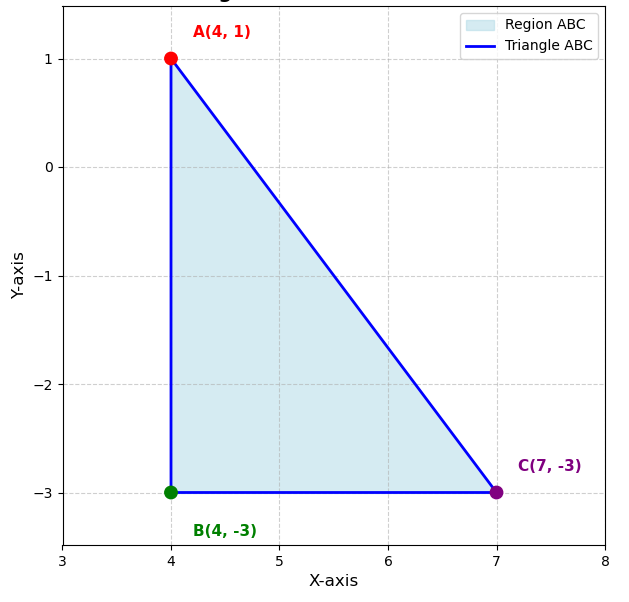
\includegraphics[width=0.6\linewidth]{/Users/unnathi/Documents/ee1030-2025/ai25btech11012/matgeo/4.8.8/figs/fig.png}
\end{center}
\end{frame}

\end{document}
